% !TEX encoding = UTF-8 Unicode

Of course, Ny$\bar{a}$ya for iPad is not the first program,  that processes expressions of propositional logic. 
Besides powerful SAT-solvers and automatic provers, which rarely can be used by beginners,
there are some applications, than can be used on a basic level.  
Most of them provide a (short) introduction to propositional logic, but they seldom offer tutorials or exercises. 	

The following overview focuses on applications accessible
per website and apps available for iPad.

\section{Websites}

\begin{itemize}
\item 
\href{http://www.cs.wfu.edu/~burg/JavaPackages/indexswingnet.html}{\bf PLogic Applet} 
by S. Lukins, A. Levicki, and 
\href{http://www.cs.wfu.edu/~burg}{J. Burg} at the
\href{http://www.cs.wfu.edu}{Wake Forest University}, is a
tutorial program for propositional logic 
“that serves a double role as an educational tool and a research environment”\footnote {
\url{http://www.cs.wfu.edu/~burg/papers/PropLogic.pdf}} and focuses 
 on interactive theorem-proving.

\item
\href{http://cl-informatik.uibk.ac.at/software/booltool/}{\bf 

\includegraphics[width=0.8cm]{clshortlogo_new.pdf}BoolTool} 
by the 
\href{http://cl-informatik.uibk.ac.at/}{Computational Logic} 
research group at the 
\href{http://informatik.uibk.ac.at}{University of Innsbruck}
“is an interface to the program BoolTool which allows the manipulation and evaluation of boolean functions.”\footnote{
\url{http://cl-informatik.uibk.ac.at/software/booltool/?page=info}}. 
It computes truth tables and binary decision diagrams and checks for satisfiability and validity.

\end{itemize}

\section{Apps for iPad}
 
Some apps for iPad or iPod touch that handle aspects of propositional logic.

\begin{itemize}

\item  \href{http://itunes.apple.com/at/app/constraints/id418722652?mt=8}{\bf 
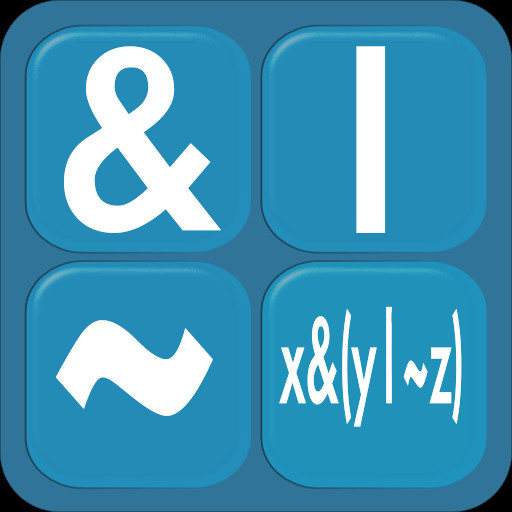
\includegraphics[width=0.8cm]{related/Constraints.png} Constraints}
by 
\href{http://www.mysvc.it/myapps/constraints/}{Davide Cucciniello} 
is a “SAT based propositional (boolean) logic engine defined by a list of models, 
where a model includes a list of constraints (a Knowledge Base) 
each defined by a propositional formula (x and (y or not z)) 
including a set of propositional (boolean) variables (x,y,z) 
and operators (and,or,not).”\footnote{
\url{http://www.mysvc.it/myapps/constraints/}} 
let's you build models in an interactive way. It also provides a short introduction in propositional logic, but no tutorials.


\item \href{http://itunes.apple.com/at/app/truth-table-generator/id507190346?mt=8}{\bf 
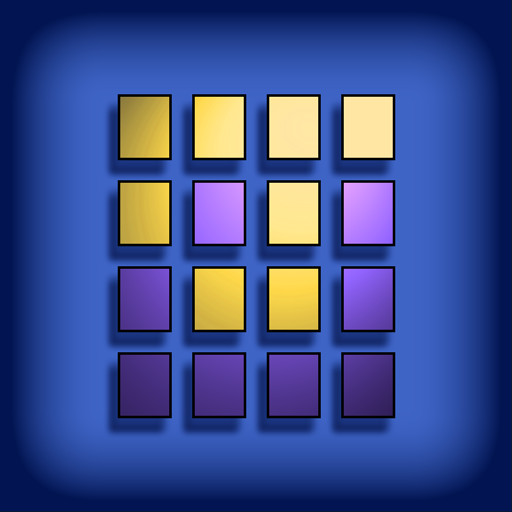
\includegraphics[width=0.8cm]{related/TruthTables.png} Truth Table Generator} 
by
\href{http://www.mertzwerkz.com/truth.html}{Mertz Werkz LLP}    
“constructs truth tables for the Boolean expressions you enter”.\footnote{
\url{http://www.mertzwerkz.com/truth.html}}
It does that nicely by using standard symbols of propositional logic (and a limited set of atoms), but nothing more.

\item
\href{http://itunes.apple.com/at/app/boolean-logic-cheat-sheet/id341959531?mt=8}{\bf 
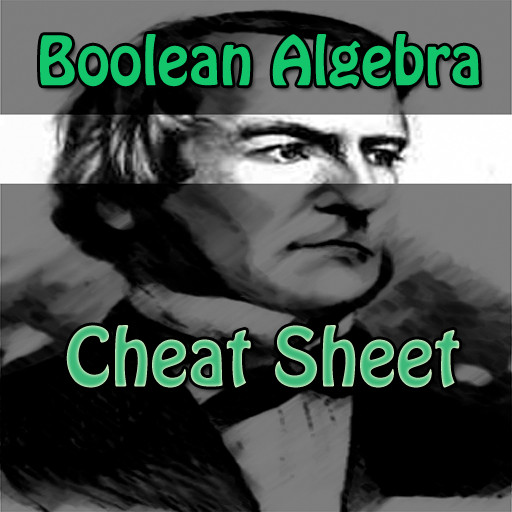
\includegraphics[width=0.8cm]{related/CheatSheet.png} Boolean Algebra Cheat Sheet} 
by 
{Clint Johnson} presents two pages of logic “rules and laws“ in low picture quality. So “all of your Boolean 
logic needs.”\footnote{
\url{http://itunes.apple.com/at/app/boolean-logic-cheat-sheet/id341959531?mt=8}} 
does not feel quite right.

\item
\href{http://itunes.apple.com/at/app/logic-mania/id434019152?mt=8}{\bf 

\includegraphics[width=0.8cm]{related/LogicMania.png} Logic Mania} 
by 
{Imagination Creations} presents seven logic gates in a list. 
Their semantics are shown in a per-gate-simulation where the user chooses the input and the app shows the result. 
A combination of gates is not possible. It's quite nice but the statement “THE [sic] reference application for students 
studying logic gates.”\footnote{
\url{http://itunes.apple.com/at/app/logic-mania/id434019152?mt=8}}
seems exaggerated.

\item
\href{http://itunes.apple.com/at/app/circuit-coder/id492180472?mt=8}{\bf 

\includegraphics[width=0.8cm]{related/CircuitCoder.png} Circuit Coder} 
by 
\href{http://sweyla.com/}{Trycycle Design HB} is a game about building digital circuits.

\end{itemize}
